\documentclass[a4paper]{usiinfbachelorproject}

\captionsetup{labelfont={bf}}
\usepackage{float}
\usepackage{amsmath}
\usepackage{graphicx}
\usepackage{enumitem}
\usepackage{booktabs}
\usepackage{hyperref}
\usepackage{listings}
\usepackage{tabularx}

\author{POLAD BAKHISHZADE}

\title{\textbf{LLM as Code-Correctness Judge}}
\subtitle{Unveiling the Causes of Large-Language-Model Failures when Assessing Java Code}
\versiondate{\today}

\begin{committee}
  \advisor[Università della Svizzera italiana, Switzerland]{ }{Gabriele}{Bavota}
  \coadvisor[Università della Svizzera italiana, Switzerland]{ }{Giuseppe}{Crupi}
\end{committee}

% ——————————————————————————— ABSTRACT
\abstract{
\textbf{Context.}  
Large Language Models (LLMs) are increasingly being used in software development tasks such as code generation, explanation, and bug fixing. An emerging frontier is the use of LLMs for code review—specifically, assessing whether a given implementation is functionally correct. This requires reasoning over both the specification and the code, making it a strong benchmark for code understanding.\\
\\[2pt]
\textbf{Objective.}  
This study investigates how the quality and quantity of natural-language context affect the ability of LLMs to assess code correctness. We ask: \emph{What kind of descriptive information helps or harms the model’s ability to judge whether a function is correct?}\\
\\[2pt]
\textbf{Method.}  
We extend the Java subset of the \textsc{CoderEval} benchmark by systematically enriching it with five structured documentation layers—ranging from brief summaries to formal pre/post-conditions. Each of 362 functions is paired with one correct and one incorrect candidate implementation. We then prompt three open LLMs—Qwen-0.5B, Qwen-1.5B, and DeepSeek-1.3B—to act as zero-shot code judges, under multiple prompt configurations.\\
\\[2pt]
\textbf{Findings.}  
The results reveal that different models respond differently to added context: smaller models benefit from concise behavioral descriptions but often degrade when presented with verbose examples or formal constraints. In contrast, larger models leverage detailed descriptions to reduce mistakes and achieve more reliable judgments. Some layers, such as examples, can introduce confusion and accuracy drop depending on the model.\\
\\[2pt]
\textbf{Outcome.}  
The study highlights the importance of model-specific prompt design and shows that more documentation is not always better. These insights can inform future systems that rely on LLMs for code quality assessment.\\
\\[2pt]
\textbf{Keywords}: LLMs; Code Review; Code Correctness; Prompt Engineering; Evaluation; Java; Dataset Enrichment
}

\begin{document}
\maketitle
\tableofcontents\newpage

% ——————————————————————————— 1 INTRODUCTION
\section{Introduction}\label{sec:intro}
Large Language Models (LLMs) such as ChatGPT~\cite{openai2023chatgpt}, GitHub Copilot~\cite{githubcopilot}, and StarCoder~\cite{li2023starcoder} have become widely adopted in software development workflows. Originally developed for general language understanding, these models have rapidly gained traction in code-related tasks, including code generation, explanation, repair, and synthesis~\cite{jiang2024survey, chen2021codex, wang2023codet}. Researchers are increasingly exploring the use of LLMs for tasks such as debugging, static analysis, and functional correctness evaluation.\\
\\[2pt]
Among the many challenges in this space, one particularly important question is whether LLMs can serve as reliable evaluators of automatically generated code. In industrial settings, such as at Google, the proportion of code written or assisted by machine learning systems is steadily increasing. However, verifying the correctness of such code remains an open problem. Traditional techniques like writing unit tests are time-consuming and require substantial human effort, creating a bottleneck in workflows that rely heavily on automated code generation. Existing automatic evaluation metrics—such as BLEU~\cite{papineni2002bleu}, ROUGE~\cite{lin2004rouge}, METEOR~\cite{banerjee2005meteor}, and BERTScore~\cite{zhang2019bertscore}—have shown significant limitations in this setting. These metrics often rely on reference implementations, which may not be available, and struggle to capture functional equivalence between semantically correct but syntactically different solutions. Recent studies also highlight flaws in applying embedding-based metrics to code-related tasks~\cite{naik2024limitations}. This motivates the need for oracle-free evaluation mechanisms capable of assessing whether a candidate implementation adheres to a given specification.\\
\\[2pt]
While LLMs have shown strong performance in code generation, an open question remains: can they also reason about the correctness of code? This question has received relatively little attention so far, as most benchmarks are designed for code generation. Moreover, adapting code generation benchmarks for correctness evaluation is not trivial. Many such benchmarks provide only minimal or vague natural language descriptions, which are insufficient to test whether a model understands the functionality of the implementation it is evaluating.\\
\\[2pt]
In this work, we investigate how the judging abilities of LLMs vary with the depth and completeness of the instructions provided. Specifically, we create a correctness evaluation benchmark by extending the \textsc{CoderEval} dataset with five levels of natural language documentation. These range from a simple one-line summary of the function's purpose (L1), to a high-level description of the expected behavior and edge cases (L2), an explanation of the function signature and its parameters (L3), concrete input/output examples (L4), and formal pre- and postconditions specifying what must hold before and after execution (L5). We evaluate three instruction-tuned models—Qwen-0.5B, Qwen-1.5B, and DeepSeek-1.3B—across 362 function–candidate pairs. Each pair is tested under two conditions: \emph{cumulative prompts}, where the model sees all levels from L1 up to a given level, and \emph{ablation prompts}, where a specific level (e.g., L4) is removed from the full prompt to isolate its impact.\\
\\[2pt]
Our results suggest that the ability of LLMs to utilize different types of documentation varies across models. For instance, Qwen-1.5B shows a modest improvement in accuracy from 50\% to 55\% when provided with more detailed prompts, indicating some benefit from richer context. In contrast, smaller models like Qwen-0.5B and DeepSeek-1.3B exhibit inconsistent performance, sometimes declining with additional information. These findings suggest that prompt design can influence model performance, but its effectiveness varies: while richer prompts help some models slightly, others show inconsistent or even worse results.

\subsection*{Report structure}

Section~\ref{sec:related} reviews related literature.  
Section~\ref{sec:design} presents our study design and dataset enrichment pipeline.  
Section~\ref{sec:results} covers results from cumulative and ablation experiments.  
Section~\ref{sec:concl} concludes and outlines future directions.

% ——————————————————————————— 2 RELATED WORK
\section{Related Work}\label{sec:related}
As Large Language Models (LLMs) gain traction in software development, a growing body of research is investigating their potential not only as code generators but also as autonomous evaluators. Yet, assessing whether a model can reliably judge the correctness of code remains an open and challenging question. This section presents an overview of related efforts, focusing on the current limitations of LLM-based evaluation and recent benchmark development.\\
\\[2pt]
A key concern raised by recent work is that LLMs often lack deep semantic understanding of their own outputs. West et al.~\cite{west2023generative} formulate this as the “Generative AI Paradox”: models that generate impressive solutions may still fail to understand them. Their findings show that even top-tier LLMs frequently make overconfident yet incorrect predictions, especially on reasoning-intensive tasks. Gu et al.~\cite{gu2024counterfeit} expand this concern in the coding domain. They construct “counterfeit” solutions—plausible-looking but incorrect code—and show that LLMs often fail to flag these as erroneous. Instead, models are easily misled by surface-level cues and rarely recover from their own failures. Collectively, these studies highlight a core insight: evaluating code correctness is fundamentally distinct from generating code. Therefore, it is not safe to assume that a model which produces plausible-looking solutions is also a reliable evaluator of such completions.\\
\\[2pt]
Several studies have designed benchmarks to assess LLMs’ judgment ability in isolation. Zhao et al.~\cite{zhao2024codejudgeeval} introduce \textsc{CodeJudge-Eval}, a benchmark where LLMs must decide whether a given candidate solution is correct. The dataset includes subtle bugs, edge cases, and misleading code snippets. Across 12 models, including GPT-4 and Claude, accuracy remained low—rarely exceeding 60\%, with GPT-4 reaching at most 65\%. These results suggest that current models struggle with code correctness as a task, regardless of their size. Zhao et al. highlight that even advanced models like GPT-4 frequently misclassify incorrect solutions that contain subtle bugs or misleading logic. They suggest that reformulating the task—by giving more precise and complete descriptions of the expected behavior—and training models using datasets that include both correct and incorrect implementations could help improve judgment accuracy.\\
\\[2pt]
An influential approach is introduced by ICE-Score from Zhuo~\cite{zhuo2023icescore}, which suggests using GPT-3.5-turbo to evaluate candidate implementations using precisely crafted prompts that focus on properties such as correctness and readability. The study shows that prompting the model to explain its reasoning before delivering a final judgment enhances alignment with human evaluations.\\
\\[2pt]
Expanding on this idea, Tong and Zhang~\cite{tong2024codejudge} develop \textsc{CodeJudge}, a framework that builds on ICE-Score’s principles through a structured, multi-step evaluation process. In this setup, two instruction-tuned models are guided through reasoning stages—including explanation and justification—before returning a binary decision on correctness. Experiments reveal significant improvements in judgment accuracy across five datasets and programming languages, particularly for smaller models like Llama-3-8B-Instruct. In our study, we build on these insights but take a different angle: instead of structuring the reasoning steps, we structure the task description itself. By layering increasingly rich information—ranging from summaries to behavioral specifications and input/output examples—we investigate whether more detailed descriptions help models act as better judges.\\
\\[2pt]
While the studies above focus on correctness, others explore how to align model judgments with human coding preferences. Weyssow et al.~\cite{weyssow2024codeultrafeedback} introduce \textsc{CodeUltraFeedback}, a dataset of 10,000 coding problems, each answered by 14 different LLMs. These outputs are then ranked by GPT-3.5 across five dimensions: style, readability, instruction-following, complexity, and explanation. The authors use these rankings as training data to fine-tune CodeLlama-7B-Instruct, teaching it to prefer responses that GPT-3.5 rated more highly. The fine-tuned model is evaluated on HumanEval+~\cite{lzi2023humanevalplus}, where it outperforms the original base model in both preference alignment and functional accuracy. Although the task focuses on stylistic and qualitative assessment rather than functional correctness, the results suggest that training with ranked outputs can guide LLMs to better evaluate and generate code along desired dimensions such as style and readability.\\
\\[2pt]
A complementary line of research examines LLMs in educational settings. Koutcheme et al.~\cite{koutcheme2025evaluating} assess whether LLMs can generate and evaluate feedback on student code submissions in introductory Python assignments. Their goal is to explore how models can assist in automated grading systems that support student learning. They find that open-source models like StarCoder2 perform competitively with proprietary models such as GPT-4, particularly when provided with annotated student submissions that include instructor-written feedback, which serve as exemplars for what good feedback should contain. While not directly focused on correctness classification, this work supports the broader feasibility of using LLMs as evaluators of code quality.\\
\\[2pt]
In summary, the field is converging on the idea that LLMs can act as judges, but only under carefully crafted conditions. While prior work has focused on benchmarks, multi-step reasoning, or feedback alignment, our study lies in incrementally enriching the prompt descriptions and examining how models with different sizes respond to varying levels of contextual detail when judging code correctness.

% ——————————————————————————— 3 STUDY DESIGN
\section{Study Design}\label{sec:design}

\subsection*{Research Question}
\noindent\textbf{RQ –} \emph{To what extent does the quality and depth of natural language documentation affect the ability of LLMs to judge the correctness of a given Java function?}

\subsection{Context: LLMs}\label{sec:llms}
We selected three instruction-tuned large language models (LLMs) of relatively small size: \textbf{Qwen2.5-Coder-0.5B-Instruct}, \textbf{Qwen2.5-Coder-1.5B-Instruct}~\cite{qwen2024report}, and \textbf{DeepSeek-Coder-1.3B-Instruct}~\cite{deepseek2024report}. These models feature approximately 0.5, 1.5, and 1.3 billion trainable parameters respectively, which is three orders of magnitude smaller than the latest foundation models such as GPT-4, estimated to exceed one trillion parameters. We chose these smaller models to balance performance and computational feasibility, allowing us to run multiple evaluations on local academic hardware without relying on large-scale infrastructure. Although computational cost was not a formal constraint of the study, using smaller models made experimentation more feasible and reproducible in standard academic settings.\\
\\[2pt]
All three models are optimized for code-related tasks and released with instruction-following tuning, meaning they have been fine-tuned to generate appropriate responses to structured natural language instructions. This makes them well-suited for prompt-based evaluation tasks like the one in this study.\\
\\[2pt]
The term \emph{“Instruct”} indicates that the model has undergone additional fine-tuning on datasets that include natural language prompts and desired completions, making it more responsive to task-specific queries. The Qwen models are part of Alibaba’s Qwen2.5 series, designed for code tasks and instruction-following scenarios. Qwen2.5-Coder models were trained on a large mixture of public and synthetic datasets, including a multilingual corpus of code, technical Q\&A, and structured programming tutorials~\cite{qwen2024report}. In particular, Qwen2.5-Coder-1.5B was optimized for multi-task code understanding and generation, and supports fine-grained control over function-level behavior through instruction tuning.\\
\\[2pt]
DeepSeek-Coder is a family of decoder-only transformer models specifically built for programming-related tasks~\cite{deepseek2024report}. The DeepSeek-Coder-1.3B variant used in our study was pre-trained on a massive 2 trillion token corpus that includes 87.5\% code and 12.5\% natural language. It was then instruction-tuned on 2 billion tokens of high-quality problem–solution pairs and user queries. The model supports over 80 programming languages and is explicitly optimized for tasks such as code completion, explanation, and functional verification, making it suitable for prompt-based correctness evaluation.\\
\\[2pt]
All models were accessed via the Hugging Face Hub\footnote{\url{https://huggingface.co}}, an open-source platform that hosts pre-trained machine learning models and provides tools for deployment and evaluation. We used the Transformers library to run the models, which handled prompt tokenization, model loading, and inference (i.e., generating predictions) through a standardized API.

\subsection{Context: Dataset}\label{sec:dataset}
We based our experiments on the Java subset of the \textsc{CoderEval} benchmark~\cite{coderEval2023}, a code generation dataset containing 230 manually curated Java programming tasks. Each task includes: (i) a natural language specification describing what the function is expected to do, (ii) a reference implementation showcasing a possible correct solution, and (iii) an associated test suite for automated correctness verification. The output of each test suite is a boolean: \texttt{pass} indicates that a candidate satisfies all test cases, while \texttt{fail} indicates that it fails at least one.\\
\\[2pt]
Before adopting all 230 tasks, we performed a thorough quality assurance procedure to ensure the reliability of the test suites. This step was crucial, as test misbehavior could bias our evaluation—for instance, by incorrectly labeling an actually wrong solution as correct.\\
\\[2pt]
We discarded 49 problems during quality control. Specifically, 20 tasks had reference implementations that failed their own test suites, indicating internal inconsistencies. Another 9 tasks had such weak test coverage that even empty functions passed all test cases. Additionally, 17 tasks were accepted by trivial dummy implementations, such as \texttt{return null;} or \texttt{return 0;}, which revealed a lack of discriminative power in the test suites. Finally, 3 tasks yielded inconsistent results for identical implementations across different evaluation runs. After filtering out these cases, we retained a final set of 181 Java tasks that passed all quality criteria and provided reliable correctness labels inferred directly from test outcomes.

\subsection{Data Collection}\label{sec:collection}

Although each problem in the dataset includes a natural language docstring, these descriptions are often minimal—typically consisting of a single vague sentence. For example: “Performs a right node rotation.”, “Skips bytes until the end of the current line.”, or “Swap values at indexes i and j in arr.”\\
\\[2pt]
Since our goal is to evaluate the extent to which the quality and depth of natural language documentation affect the ability of LLMs to judge the correctness of a given Java function, the one-line documentation featured in the \textsc{CoderEval} dataset is insufficient to answer this question. For this reason, we augmented the description of each code generation problem with a five-layer natural language description covering different aspects of code documentation, such as parameter explanations and examples of input–expected output pairs.

\subsubsection{Augmenting the Dataset}\label{sec:augmentation}
Our goal is to study the extent to which the natural language documentation affect the ability of LLMs to judge the correctness of Java functions. To enable this evaluation, we enriched the \textsc{CoderEval} dataset with additional structured documentation, since the original format was designed for code generation, not understanding.\\
\\[2pt]
We used GPT-4o to produce this documentation because it was both scalable and accurate. Manual annotation of all 181 Java functions across multiple levels would have been impractical, and GPT-4o consistently followed structured formatting and stylistic constraints when prompted correctly.\\
\\[2pt]
Each prompt to GPT-4o included the full Java function body and its name. The model was asked to return a five-part structured description covering different semantic aspects of the function:

\begin{enumerate}[leftmargin=15pt]
  \item[\textbf{L1}] \textbf{Summary}: a concise one-sentence description of the function's high-level purpose, strictly excluding edge cases.
  \item[\textbf{L2}] \textbf{Behavioral description}: a 1--2 sentence narrative detailing the function’s logic, including how edge cases and special conditions are handled.
  \item[\textbf{L3}] \textbf{Signature explanation}: structured tags describing the meaning of each parameter and the return value (\texttt{@param}, \texttt{@return}, \texttt{@throws}), if applicable.
  \item[\textbf{L4}] \textbf{Examples}: several one-line input–output pairs with explanatory notes clarifying expected behavior.
  \item[\textbf{L5}] \textbf{Preconditions and postconditions}: short logical statements capturing required input constraints and expected output guarantees.
\end{enumerate}
The outputs followed a fixed format and were manually verified for quality and correctness. We ensured that L1 remained high-level, L2 captured the full logic and edge cases, and L3–L5 remained accurate, relevant, and specific to each function.\\
\\[2pt]
This enrichment gave us modular “building blocks” that could be flexibly combined into prompts with different levels of information. For example, combining L1 and L2 produces a compact explanation of the function’s purpose and behavior, while L1 and L3 give purpose plus interface-level understanding without relying on examples or full logic. This modularity was essential for constructing the incremental and layer-removal settings used in our evaluation.\\
\\[2pt]
To make this enrichment structure more concrete, we present a full example based on one of the tasks from the dataset.

\begin{lstlisting}[language=Java, caption={Reference implementation of \texttt{trimArrayElements}}, label={lst:trim}]
public static String[] trimArrayElements(String[] array){
  if (Objects.isEmpty(array)) {
    return new String[0];
  }
  String[] result = new String[array.length];
  for (int i = 0; i < array.length; i++) {
    String element = array[i];
    result[i] = (element != null ? element.trim() : null);
  }
  return result;
}
\end{lstlisting}
The original \textsc{CoderEval} docstring was:

\begin{flushleft}
\ttfamily
\small
/\** \\
Trim the elements of the given String array, calling String.trim() on each of them.\\
@param array the original String array\\
@return the resulting array (of the same size) with trimmed elements\\
*\ /
\end{flushleft}
Below is the five-layer enrichment produced using GPT-4o:\\
\\[2pt]
\textbf{L1 – Summary:} Trims whitespace from each element of an array.\\[2pt]
\textbf{L2 – Behavioral description:} Trims leading and trailing whitespace from each string in the input array. If the array is null, returns an empty array. If an element is null, it remains null in the output.\\[2pt]
\textbf{L3 – Signature explanation:}
\begin{quote}\ttfamily
@param array String[]: The input array of strings to be trimmed.\\
@return String[]: A new array with trimmed strings, or nulls where applicable.
\end{quote}
\textbf{L4 – Examples:}

\begin{center}
\renewcommand{\arraystretch}{1.2}
\begin{tabular}{@{}l@{\hskip 1em}l@{}}
\texttt{\{ "  hello ", " world " \}} \textrightarrow\ \texttt{\{ "hello", "world" \}} & (trims spaces) \\
\texttt{\{ "foo", "bar" \}} \textrightarrow\ \texttt{\{ "foo", "bar" \}} & (no trimming needed) \\
\texttt{null} \textrightarrow\ \texttt{\{\}} & (handles null input)
\end{tabular}
\end{center}
\textbf{L5 – Preconditions and postconditions:} Input may be null or contain null elements. Output array has the same length as input; each non-null string is trimmed, nulls are preserved.



\subsubsection{Building Candidate Pairs}\label{sec:judgments}
To evaluate whether LLMs can judge the functional correctness of code based on natural language descriptions, we paired each of the 181 Java problems with two candidate implementations: one correct and one incorrect. These implementations were not drawn from \textsc{CoderEval} itself, but were generated by us using several large language models, including DeepSeek-Coder-6.7B~\cite{deepseek2024report} and Qwen2.5-Coder-7B~\cite{qwen2024report}. We generated multiple candidate solutions for each problem and compiled them into a custom knowledge base of over 5,000 Java implementations.\footnote{\url{https://github.com/poladbachs/Bachelor-Thesis/blob/main/CoderEval/knowlbase_codereval.csv}}\\
\\[2pt]
We applied a filtering process to remove trivial, duplicate, or unusable code. First, we discarded placeholder code such as \texttt{/* implementation goes here */} or empty function bodies, which clearly lacked any executable logic. Second, we excluded logic-less shells like \texttt{return;} or \texttt{return 0;} that performed no computation and could not plausibly be evaluated for correctness. Third, we removed print-only stubs such as \texttt{System.out.println("TODO");}, as these were clearly placeholders and not real attempts at implementation. Fourth, we eliminated duplicate implementations to ensure that each candidate pair provided a distinct comparison case. Finally, we removed candidates that relied on methods, classes, or functionality not defined within the task scope. For example, some generated implementations contained comments such as:
\begin{quote}\ttfamily\small
// Assuming there's a getDefaultValue method for the class\\
// Assuming IsomorphicGraphMapping is a custom class\\
// Update heights (assuming that updateHeight() is defined)
\end{quote}
Such phrases indicate that the code presumes the existence of external dependencies that are not guaranteed to be available within the function's context. Including these candidates would introduce ambiguity, as correctness could no longer be determined purely based on the prompt and provided code. We therefore excluded all such cases to maintain a closed-world evaluation setup, where all necessary information is explicitly present.\\
\\[2pt]
After filtering, we finalized the dataset by selecting one correct and one incorrect implementation per problem. When no valid correct candidate was found, we fell back to using the original reference implementation from \textsc{CoderEval}. In two exceptional cases where no usable incorrect candidates were available, we manually inserted a faulty variant into the dataset to complete the correct–incorrect pairing.

\subsection{Prompting and Evaluation Setup}\label{sec:evaluation}
Each model was tasked with a binary classification problem: given a natural language description, a function signature, and a candidate implementation, it must decide whether the implementation correctly satisfies the described behavior. The model outputs \texttt{1} if the implementation is correct, and \texttt{0} otherwise.
The exact prompt given to the models was formatted as follows, using placeholders to insert task-specific information:

\begin{quote}\ttfamily
You will be provided with the description ("Description") and the signature ("Signature") of a Java function to implement. You will also see a candidate implementation ("Candidate"). Your role is to evaluate the correctness of the Candidate, providing as output either 0 or 1, and no other text:

0. Wrong Implementation: The implementation does not correctly implement the described function.\\
1. Correct Implementation: The implementation correctly implements the described function.

\# Description:\\
- Summary: \{L1: one-line summary\}\\
- Behavior: \{L2: behavioral explanation\}\\
- Signature Description: \{L3: @param/@return tags\}\\
- Examples: \{L4: input–output pairs with notes\}\\
- Preconditions and Postconditions: \{L5: logical constraints\}

\# Signature:\\
\{First line of candidate code\}

\# Candidate:\\
\{Full candidate implementation\}

\# Output:
\end{quote}
All prompts were encoded and passed to the models using Hugging Face Transformers with temperature set to 0.2. This low temperature was chosen to reduce randomness, since we could not afford to run multiple evaluations on the same instance. A limit of \texttt{max\_new\_tokens = 20} was enforced to constrain output length and prevent verbose completions, as the task only required a single-digit response (0 or 1). Model outputs were parsed to extract a binary classification, and any non-conforming output was treated as invalid and recorded as \texttt{None}.\\
\\[2pt]
We evaluated model performance under two experimental settings. In both, the baseline was the minimal prompt containing only the L1 summary layer.\\
\\[2pt]
In the first setting, prompt enrichment, we incrementally increased the amount of documentation information provided to the model. Starting from L1 alone, we progressively added layers in the following order: L2 (behavioral explanation), L3 (signature-level tags), L4 (input–output examples), and finally L5 (logical constraints). This yielded five prompt configurations per model, corresponding to L1, L1+L2, L1+L2+L3, L1+L2+L3+L4, and the full L1–L5 stack. We applied this setup to three LLMs—Qwen-0.5B, Qwen-1.5B, and DeepSeek-1.3B—resulting in 15 enrichment experiments in total.\\
\\[2pt]
In the second setting, layer removal, we started from the full prompt containing all five documentation layers (L1–L5) and selectively removed individual or combined layers to assess their individual effect on model performance. Rather than exhaustively testing all combinations, we defined a limited set of configurations per model to observe the contribution of each layer. This experimental approach helped isolate which layers had the greatest impact on accuracy and whether some components could be omitted without harming performance. The detailed discussion of results is presented in Section~\ref{sec:results}.

\subsection{Data Analysis}\label{sec:analysis}

Each model was evaluated on a binary classification task: given a natural language description of a Java function and a candidate implementation, decide whether the implementation correctly satisfies the described behavior. Ground truth correctness labels were drawn from the dataset: each candidate was pre-labeled as either correct or incorrect. Separately, the model was instructed to output \texttt{1} if it judged the implementation to be correct, and \texttt{0} if it judged it to be incorrect.\\
\\
Using these two independent sources—predefined correctness labels and model predictions—we computed standard confusion matrix metrics. A true positive (TP) occurs when the model correctly identifies a correct implementation. A true negative (TN) is when the model correctly identifies an incorrect implementation. A false positive (FP) occurs when the model mistakenly labels an incorrect implementation as correct, and a false negative (FN) when the model fails to recognize a correct implementation.\\
\\[2pt]
Because our dataset was balanced—containing 181 correct and 181 incorrect implementations—we report accuracy as the primary performance metric. Accuracy reflects the overall proportion of correct classifications (TP and TN) over all evaluated samples:
\[
\text{Accuracy} = \frac{TP + TN}{TP + TN + FP + FN}
\]
Model outputs that did not include a valid binary prediction (\texttt{0} or \texttt{1}) were marked as invalid and excluded from metric calculations.


\subsection{Replication Package}\label{sec:replication}
All source code, enriched datasets, model evaluation scripts, and plotting tools are available in the following GitHub repository:
\begin{center}
\url{https://github.com/poladbachs/Bachelor-Thesis}
\end{center}
The repository includes all CSVs, accuracy plots, confusion matrices, and detailed README instructions for full optional replication. Environment dependencies are specified in \texttt{requirements.txt}.

% ——————————————————————————— 4 RESULTS
\section{Results \& Discussion}\label{sec:results}

\subsection{Incremental Enrichment (L1 $\rightarrow$ L5)}

To assess how progressively detailed documentation impacts model performance, we first examine the cumulative enrichment results shown in Figure~\ref{fig:acc-l1-l5}. Each model was evaluated across five prompt variants, from the minimal summary-only setting (L1) to the full specification (L1–L5), revealing distinct behavioral patterns across models.
\begin{figure}[H]\centering
  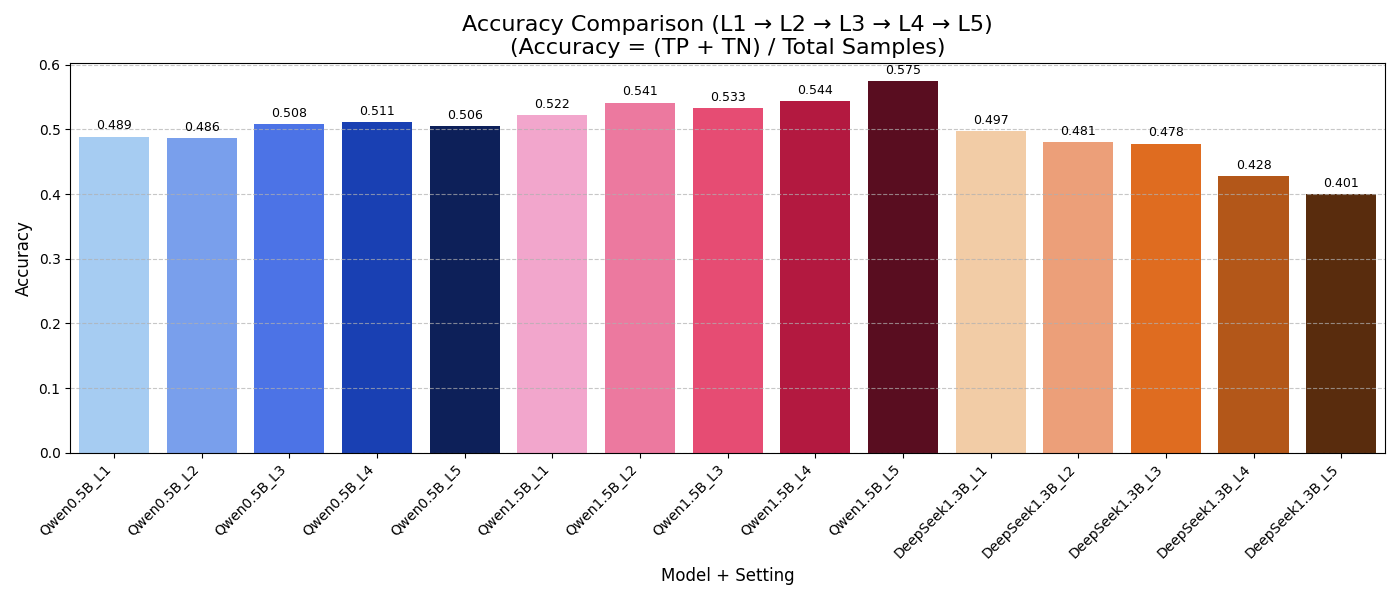
\includegraphics[width=0.95\linewidth]{figures/accuracy_comparison.png}
  \caption{Accuracy comparison across cumulative prompt settings. Each model is tested from L1 to L5.}
  \label{fig:acc-l1-l5}
\end{figure}
\noindent
The smallest model, Qwen-0.5B, starts at an accuracy of 0.489 with only the summary (L1) and fails to gain meaningful improvement through L2. However, accuracy rises once signature explanations (L3) and concrete examples (L4) are introduced, reaching a peak of 0.511. The final documentation layer (L5), which introduces formal logical conditions, causes a slight performance drop. This pattern suggests that Qwen-0.5B benefits from moderate enrichment, particularly when structural or procedural cues are provided, but may be overwhelmed by overly formal content. \\
\\
Qwen-1.5B, with three times the parameter count of 1.5 billion, exhibits a markedly different trajectory. It improves with each successive layer, achieving 0.575 accuracy at L5. The gains are smooth and incremental but remain modest overall, indicating that while this model is capable of integrating richer, layered context, the improvement is limited in absolute terms. Notably, there is a slight dip at L3, where performance temporarily decreases before recovering with L4 and L5. This suggests that method signature descriptions may introduce redundancy or noise that momentarily disrupts the model's internal reasoning. Unlike Qwen-0.5B, however, Qwen-1.5B shows no degradation with the introduction of preconditions or postconditions, suggesting a higher tolerance for semantic complexity. \\
\\
In contrast, DeepSeek-1.3B follows a declining trajectory. It reaches its highest accuracy of 0.497 under the minimal L1 prompt, but performance drops steadily with each additional layer, falling to 0.401 at L5. Unlike the Qwen models, DeepSeek does not benefit from richer documentation. Instead, the added layers appear to introduce noise or distraction. The consistent decline suggests that the model struggles to integrate compositional prompt structure and performs best when given minimal, straightforward input.

\subsection{Model Behavior via Confusion Matrix Metrics}
To better understand these contrasting dynamics, we inspect the confusion matrix decomposition of model predictions across the enrichment levels. Figures~\ref{fig:qwen05-matrix},~\ref{fig:qwen15-matrix}, and~\ref{fig:deepseek-matrix} report true positives (TP), true negatives (TN), false positives (FP), and false negatives (FN) for Qwen-0.5B, Qwen-1.5B, and DeepSeek-1.3B respectively.
\begin{figure}[H]\centering
  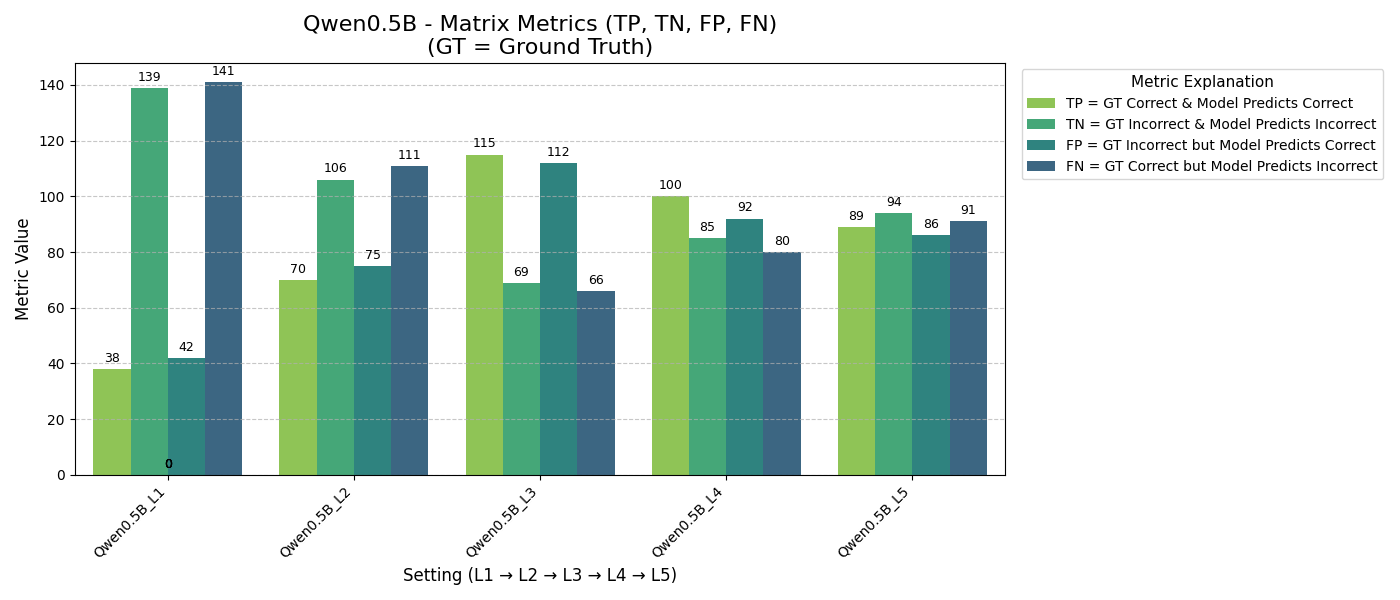
\includegraphics[width=\linewidth]{figures/Qwen0.5B_matrix_metrics.png}
  \caption{Confusion-matrix metrics for Qwen-0.5B across L1 to L5.}
  \label{fig:qwen05-matrix}
\end{figure}
\noindent
Qwen-0.5B initially misclassifies a large number of correct implementations as incorrect at L1 and L2, as reflected in the high false negative counts (141 and 111, respectively). This indicates that the model lacks sufficient information to identify correctness with only a summary (L1) or a behavioral description (L2). At L3, where signature information is added, false negatives drop substantially (to 66), and true positives increase sharply, suggesting that even lightweight structural context (e.g., signature description) provides actionable cues. At L4, true positives slightly decline (to 100), and false negatives rise again, indicating some loss in the model's ability to detect correct code. Meanwhile, true negatives increase (to 85), suggesting that the examples may help the model reject incorrect implementations more reliably. At L5, true positives decline while true negatives and false negatives rise, indicating that the model becomes more conservative and hesitant to label candidates as correct. Overall, Qwen-0.5B performs best when given mid-level semantic structure (L2 and L3), but its decision boundary shifts unfavorably as deeper enrichment is added, reducing its ability to recognize correct code without improving classification of incorrect ones.
\begin{figure}[H]\centering
  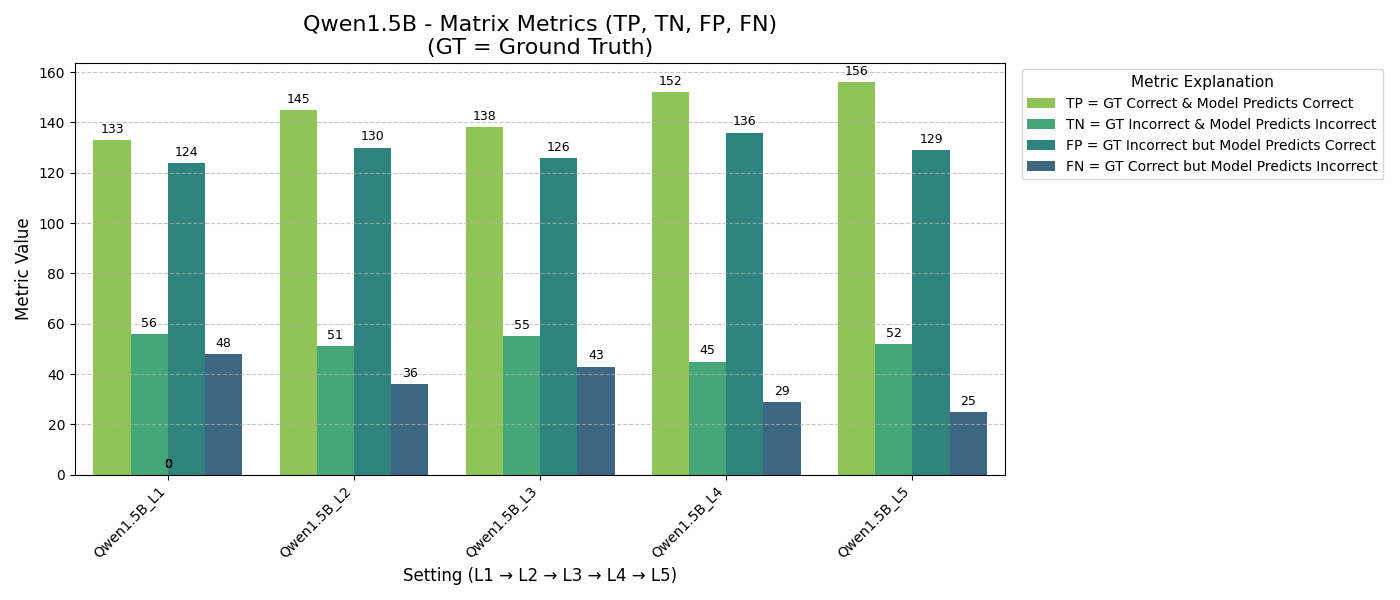
\includegraphics[width=\linewidth]{figures/Qwen1.5B_matrix_metrics.png}
  \caption{Confusion-matrix metrics for Qwen-1.5B across L1 to L5.}
  \label{fig:qwen15-matrix}
\end{figure}
\noindent
Qwen-1.5B consistently improves as more documentation is added, with true positives increasing from 133 at L1 to 156 at L5, and false negatives dropping from 48 to 25. This trend indicates that the model is increasingly able to identify correct implementations with additional context. However, a clear deviation is observed at L3: true positives dip from 145 (L2) to 138, while both true negatives and false negatives increase. This suggests that the signature-level information in L3 introduces noise or ambiguity, disrupting the positive trend. After L3, performance recovers, and the model resumes its upward trajectory. Meanwhile, false positives increase slightly across layers from 124 to 129, suggesting that the model becomes slightly more permissive in labeling incorrect code as correct. While this increase is modest, it implies a mild trade-off: the model becomes better at recognizing valid code but at the cost of a slight increase in overacceptance. Notably, the gain in true positives outweighs the false positive drift, resulting in an overall improvement in performance. Unlike Qwen-0.5B, the smallest model in our study with 0.5 billion parameters, Qwen-1.5B appears to integrate new layers effectively and continues to benefit from full enrichment, though not all layers contribute equally to its final performance.
\begin{figure}[H]\centering
  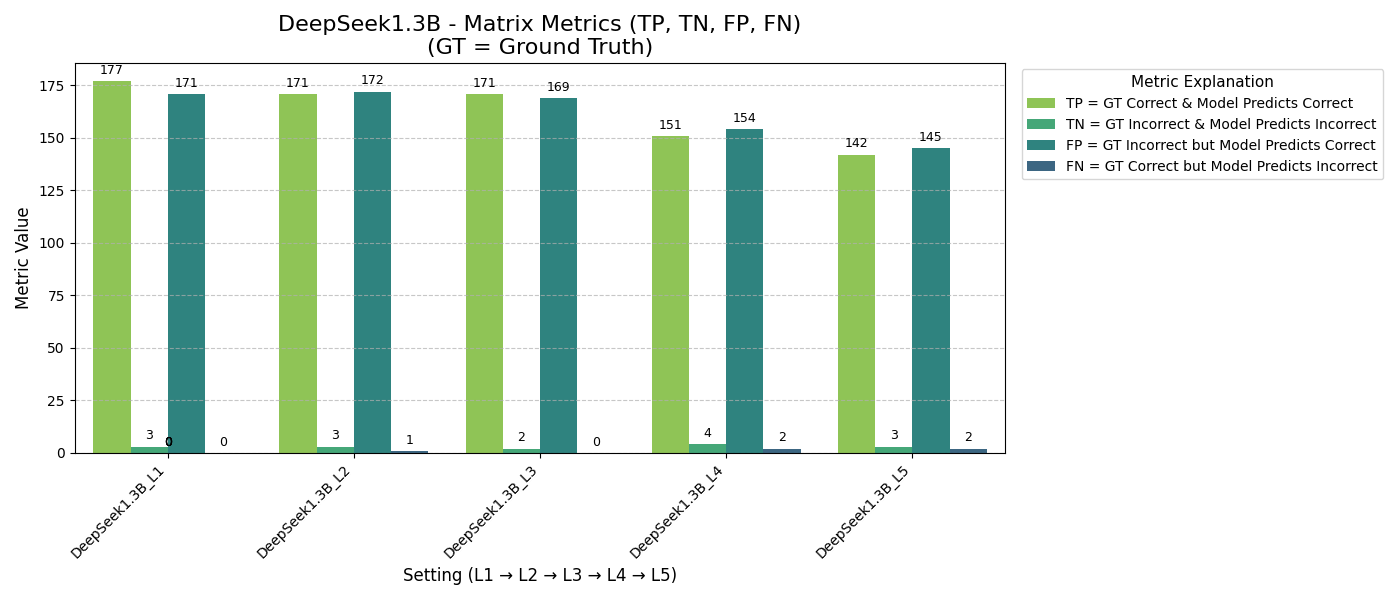
\includegraphics[width=\linewidth]{figures/DeepSeek1.3B_matrix_metrics.png}
  \caption{Confusion-matrix metrics for DeepSeek-1.3B across L1 to L5.}
  \label{fig:deepseek-matrix}
\end{figure}
\noindent
DeepSeek-1.3B exhibits a distinct behavior compared to the Qwen models. From L1 to L3, both true positives and false positives remain consistently high (above 170), indicating that the model classifies nearly all implementations as correct—whether they are actually correct or not. This reflects a clear tendency to always predict "1", showing that DeepSeek fails to distinguish between correct and incorrect code when the prompt includes only limited documentation (L1 to L3). True negatives and false negatives, in contrast, stay near zero, showing that the model struggles to recognize incorrect implementations. However, at L4 and L5, both true positives and false positives decline noticeably—not due to improved selectivity, but because the model increasingly fails to produce a valid binary output. This increase in non-responses (i.e., outputs other than 0 or 1 are classified as None and not included in metrics) highlights DeepSeek's difficulty in handling verbose or highly structured prompts. The added complexity does not confuse its decision boundary directly, but rather overwhelms it to the point of non-commitment. Overall, DeepSeek is overly accepting at low layers of documentation and increasingly silent at higher enrichment levels, undermining its reliability as a code judge under detailed input.

\subsection{Single-Layer Removal Analysis}

Having assessed cumulative enrichment, we now isolate the impact of individual layers through selective removal from the full L1 to L5 prompt. Figure~\ref{fig:ablation-accuracy} displays the resulting accuracy values after omitting one documentation level at a time.
\begin{figure}[H]\centering
  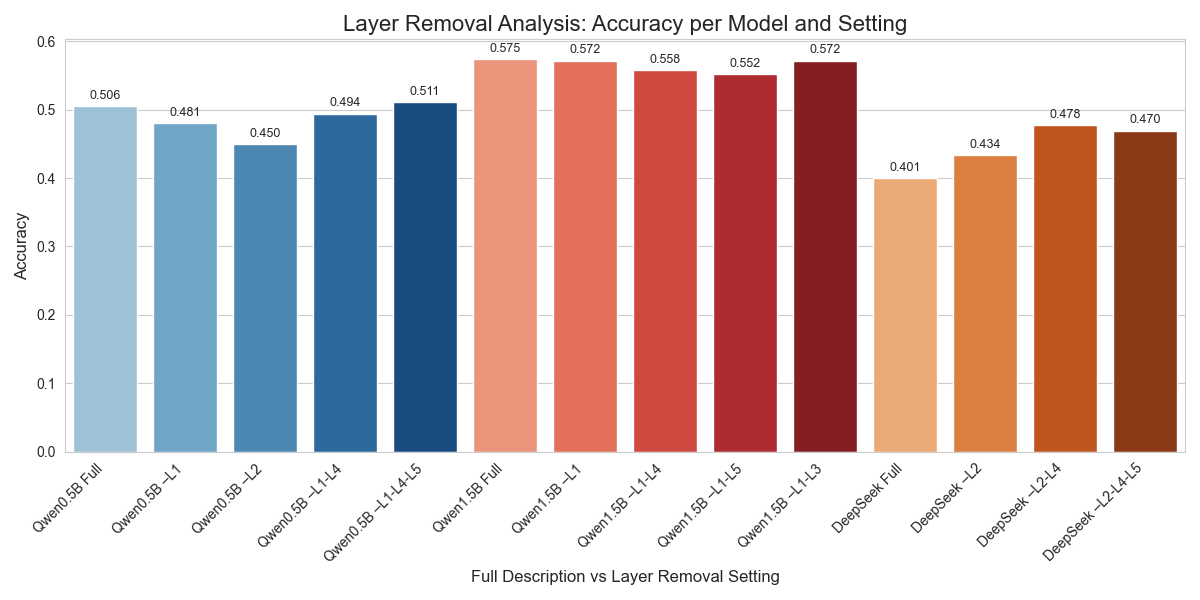
\includegraphics[width=0.95\linewidth]{figures/ablation_accuracy.png}
  \caption{Accuracy after removing selected layers from the full prompt.}
  \label{fig:ablation-accuracy}
\end{figure}
\noindent
Removing the behavioral layer (L2) causes the most significant accuracy drop for Qwen-0.5B, reducing performance from 0.506 to 0.450. This confirms that mid-level functional cues are central to the model's success. Interestingly, removing the summary (L1) has a minor effect, suggesting that Qwen-0.5B does not depend heavily on introductory one-liner, since it already has a detailed description (L2). \\
\\
Qwen-1.5B, in contrast, maintains high accuracy regardless of which individual layer is removed. The worst-case drop—removing L4—only reduces accuracy from 0.575 to 0.558. This demonstrates that no single layer is essential for the model to perform well and suggests that Qwen-1.5B can extract sufficient meaning from the remaining context when any one component is missing. Notably, removing L1 has almost no effect, confirming that this summary layer is redundant at this model size. For this reason, we exclude L1 in all compound removal scenarios and instead focus on testing the impact of removing richer content (L4, L5) under a reduced setting. The findings here support the view that Qwen-1.5B integrates context holistically and remains robust under prompt variation, even when trimmed. \\
\\
DeepSeek again stands out. Its full prompt accuracy is lowest (0.401), while selective removals such as –L2, –L2L4, or –L2L4L5 improve accuracy incrementally. This pattern suggests that DeepSeek struggles with verbosity or structural redundancy and performs better under minimalistic settings that reduce distractive context.

\subsection{Compound Layer Removal}

To assess how interactions between layers influence model behavior—and to investigate whether some components might be removed without degrading performance—we evaluate selected compound removals. These tests explore how combinations of omitted documentation layers affect final accuracy under the full prompt setting (L1–L5), as shown in Figure~\ref{fig:ablation-accuracy}. \\
\\
For Qwen-0.5B, the best-performing configuration emerges not from cumulative enrichment, but from selective reduction. Removing only Layer 1 (summary) or Layer 2 (behavioral spec) results in a performance drop—down to 0.481 and 0.450 respectively—demonstrating that both layers are comparatively important. However, when Layers 1 and 4 are removed together, accuracy recovers to 0.494, approaching the full prompt baseline of 0.506. Most notably, when Layers 1, 4, and 5 are excluded—leaving only the behavioral and signature layers (L2 and L3)—accuracy increases to 0.511, the model's highest score. This indicates that Qwen-0.5B operates best under a focused prompt structure: L2 provides actionable intent, and L3 supplies signature framing. Additional narrative, examples, or formal logic appear to interfere with rather than enhance performance. \\
\\
In Qwen-1.5B, we begin compound removal by discarding L1, which has already been shown to be redundant in single-layer analysis. Once L1 is excluded, we assess the contribution of L4 and L5 through two combinations: -L1L4 and -L1L5. Both lead to a slight performance drop—from 0.575 to 0.55 and 0.55 respectively—confirming that while examples (L4) and logical constraints (L5) are not essential, they still offer a modest benefit. We then reintroduce L4 and L5 and instead remove L1 and L3. The result remains 0.57, nearly identical to the full prompt. This confirms that L3, like L1, is not contributing meaningfully to final performance. Overall, the model's best performance is achieved with all layers present, but L1 and L3 can be omitted without any loss, while L2, L4, and L5 form the core of its effective reasoning. \\
\\
DeepSeek-1.3B exhibits the clearest improvement under compound removal. Its accuracy increases from 0.401 to 0.478 when both the behavioral spec (L2) and the example list (L4) are removed. A similar trend holds for the –L2L4L5 setting (0.470). These results confirm that DeepSeek struggles with verbose or compositional prompts and benefits from minimized input. For this model, Layers 2 and 4 likely introduce phrasing or detail that distracts rather than guides its decision-making. This may be because L4 always presents idealized, successful outputs, encouraging the model to generalize too confidently, while L2 conveys intent in a more informal and stylistic tone than the strict logical constraints in L5. Their combination may introduce conflicting internal cues, leading to unstable or overly permissive decisions. \\
\\
These findings confirm that documentation layer utility is highly model-specific. DeepSeek benefits most from minimal structure, Qwen-0.5B from targeted specification, and Qwen-1.5B from full enrichment. Notably, the strongest-performing model is also the most flexible: Qwen-1.5B retains high accuracy even when limited layers such as the summary (L1) or method signature (L3) are omitted, indicating that these inputs contribute little beyond the richer behavioral and logical cues such as L2 and L4. Effective prompt design should therefore consider model size—i.e., the number of parameters—when determining how much detail to include.

\section{Conclusions \& Future Work} \label{sec:concl}

This study set out to explore how different types of natural language documentation influence the ability of language models to judge the functional correctness of Java code. Motivated by the observation that existing datasets provide minimal supervision, we constructed an evaluation pipeline that progressively enriched function descriptions with five layered components—ranging from simple summaries to formal preconditions and postconditions. We then examined how three instruction-tuned LLMs of varying size—Qwen-0.5B, Qwen-1.5B, and DeepSeek-1.3B—responded to these prompt variants in both cumulative and subtractive (layer removal) conditions. \\
\\
Across 362 candidate pairs, we evaluated each model's binary judgments using accuracy and confusion matrix analysis. The results showed that prompt effectiveness is not uniform but deeply model-dependent. Qwen-0.5B benefited most from lightweight yet specific input: it achieved peak performance when provided only with the behavioral specification and the method signature (L2+L3), while further enrichment with examples and logical constraints introduced noise and reduced reliability. In contrast, Qwen-1.5B demonstrated robust improvements across the full prompt hierarchy, tolerating verbosity and integrating context holistically. Interestingly, DeepSeek-1.3B exhibited the opposite trend: its performance degraded with each added layer, and it reached peak accuracy only under compound removals that eliminated verbose or stylistically conflicting elements. \\
\\
In practical terms, these results suggest that prompt design must be carefully tailored to each model. Qwen-0.5B, the smallest model in our evaluation, performed best with focused prompts containing only behavioral descriptions (L2) and method signatures (L3). When enriched with additional layers such as one-line summaries (L1), examples (L4), or formal pre/post constraints (L5), performance declined—indicating that the model struggled to extract meaningful cues from verbose or surface-level documentation.\\
\\
Qwen-1.5B, in contrast, was more tolerant to prompt verbosity and continued to perform well even when enriched with less critical layers. It benefited modestly from examples and constraints, and maintained high accuracy even when the summary or signature information was removed. These findings show that optimal prompt construction is not universal: models differ in what information they can effectively use. Designing effective prompts requires awareness of the specific model's behavior and how it responds to different types of documentation.

\subsection*{Future Work}
Several directions remain open for future exploration. First, our evaluation was static: models were asked to classify correctness using fixed input pairs, without follow-up clarification or iterative reasoning. Future work could investigate dynamic prompting strategies, such as presenting labeled examples before classification or incorporating intermediate feedback signals—e.g., using model confidence scores or tool-generated hints—to guide the model during the decision process. \\
\\
Second, our correctness labels were based strictly on the test suite's exit code. While this was appropriate for a binary classification task, it does not capture cases of subtler distinctions. For instance, a candidate might solve the main use cases correctly but fail on rare edge conditions (\textit{partial correctness}), or implement the same functionality using a different structure or algorithm (\textit{alternative valid implementations}). Similarly, some candidates may be correct but written in inefficient or hard-to-read styles (\textit{stylistic diversity}). Future evaluations could explore more nuanced supervision signals. For example, \textit{semantic equivalence scoring}—as explored in CodeXGLUE~\cite{Lu2021codexglue}—compares the behavior of two programs across a diverse set of inputs rather than relying on a fixed test suite. Alternatively, \textit{human-in-the-loop evaluation} could involve expert annotators scoring implementations on correctness, clarity, and style, providing richer feedback than correct/incorrect outputs alone~\cite{smith2021human}. \\
\\
Third, our analysis focused on three small to moderately sized open models due to resource constraints. Including larger models, such as GPT-4 or Claude (Anthropic's large language model~\cite{claude2023blog}), could clarify whether the trends we observed generalize to higher-capacity systems or are unique to the models tested here.\\
\\
Finally, additional research could examine failure patterns in more detail—for instance, when and why specific layers like L4 or L5 confuse a model. Understanding such breakdowns could help define safer and more effective prompt templates for future applications in code assessment or feedback generation.\\
\\
In conclusion, this study demonstrates that not all layers of natural language documentation contribute equally to model accuracy. Some forms of enrichment help even though still moderately, while others may dilute or obscure the underlying intent. Prompting strategies should therefore be designed with model-specific behaviors in mind, not based on the assumption that more detail always leads to better results.\\

% ——————————————————————————— REFERENCES
\bibliographystyle{abbrv}
\bibliography{references}

\end{document}